full pipeline testing 

Accuracy, time and translation under fully efficient conditions

test with low time constraints

test with low accuracy constraints

output runtime per image in both gps, and no gps stages



comment on applicability
comment on dynamic camera parameter inference

comment on generalizability




test with lower resolution 

test with crop

show path visuals: expected vs real path, scaled image with DOT 
xxx - i said stress tests were done at lower res



Basically look at runtime per image in add phase, inference phase, and loss phase

GPS path estimate

What i want

Time needs to be per addition and per inference and per add x 
Baseline performance
overall best pipeline: accuracy, time, robustness x
efficient mode: time, robustness NO
accurate mode: accuracy, robustness NO

Nice looking results:
Heat map (1, 7 bin) x and y separate, and radial - X 
GPS (or not and pixel) path estimate (ADD BACK NEXT ITERATION)
dataset specific clouds - X


Stress testing:
overlap testing : test under crops (ie 50\% overlap, 25\% overlap, 10\% overlap) and see how it affects the pipeline. (ADD COVERAGE TOO)
blur testing (NOT YET)


observations:
20/30 pixel off - 100-120m off, 

hold space 5-6 - can drop?





efficiency mode: 
global: 1200, rot: 2000, loc, 2400


normal mode: 
global: 2000, rot: 3000, loc, 3000







% % last dataset update
% Dataset: DATSETAMAZ
% Linear regression inferred factor x: 3.3738789378321217
% Linear regression inferred factor y: 3.455327073764407

% Interm angle: -0.0000 deg, DEV-X,Y (pixels): (-2.1586038122612763, 4.334424096596138)
% Interm angle: -195.4006 deg, DEV-X,Y (pixels): (-0.2604724435900607, -29.182543542776898)
% Interm angle: -181.0718 deg, DEV-X,Y (pixels): (-8.726932834933166, -12.225699582213906)
% Interm angle: -181.1089 deg, DEV-X,Y (pixels): (8.904814054491197, 11.030645800864932)
% Interm angle: -181.0718 deg, DEV-X,Y (pixels): (0.9801064092702632, 15.303823953695769)
% Interm angle: -181.0433 deg, DEV-X,Y (pixels): (8.748992422901125, -19.72505001809168)
% Interm angle: -3.4582 deg, DEV-X,Y (pixels): (3.2180113388305926, 15.783338928629199)
% Interm angle: -46.8223 deg, DEV-X,Y (pixels): (-26.097384699788336, 27.490768506720798)
% Interm angle: -27.1818 deg, DEV-X,Y (pixels): (20.319732604609385, 5.860656102103292)
% Interm angle: 3.2985 deg, DEV-X,Y (pixels): (-21.085862010385313, 7.309995745239746)
% Interm angle: -27.1818 deg, DEV-X,Y (pixels): (14.764122295494133, -6.466321846361325)
% Interm angle: 3.2985 deg, DEV-X,Y (pixels): (-8.075413783313135, -10.244650151048972)
% Interm angle: 20.5317 deg, DEV-X,Y (pixels): (-15.580909035827062, 21.877502015975864)
% Mean_Add_Time: 0.5866720517476399, Mean_Parameter_Inference_Time: 1.158870315551758, Mean_Location_Inference_Time: 1.4756297331589918
% Var_Add_Time: 0.03303354394583544, Var_Parameter_Inference_Time: 0.00388432902635941, Var_Location_Inference_Time: 0.005121094337363578
% Total Time: 33.77761888504028
% Percentage Deviation: [2.7132406] %
% Preprocessing Global Detector: ORB, Preprocessing Global Matcher: FLANN, Global Matching Technique: Histogram, Local Detector: AKAZE, Local Matcher: FLANN
% Mean Absolute Error GPS: [12.52910685]
% [17.90947287]
% Mean Length of Global Keypoints: 5175.8
% Mean Number of Loc good Matches: 1477.1666666666667
% Mean Number of Global good Matches: 543.3555555555556
% Time taken to execute The Method: 37.2754 seconds




\section{Baseline Results}

\begin{table}[H]
    \centering
    \caption{Performance Metrics Across Datasets}
    \label{tab:Optimal_Method_Metrics}
    \begin{tabular}{|c|c|c|c|c|c|}
    \hline
    \textbf{Metric} & \textbf{CITY1} & \textbf{CITY2} & \textbf{ROCKY} & \textbf{DESERT} & \textbf{AMAZON} \\ \hline
    \textbf{RMSE GPS Error (m)} & 55.09 & 8.56 & 19.15 & 31.44 & 30.37 \\ \hline
    \textbf{Percentage GPS Deviation (\%)} & 5.09 & 0.80 & 2.13 & 3.54 & 4.75 \\ \hline
    \makecell{\textbf{Mean Add Time} \\ \textbf{(s)}} & 0.655 & 0.722 & 0.644 & 0.505 & 0.632 \\ \hline
    \makecell{\textbf{Mean Parameter\\Inference Time (s)}} & 1.624 & 1.420 & 2.052 & 1.232 & 1.357 \\ \hline
    \makecell{\textbf{Mean Location\\Inference Time (s)}} & 2.112 & 1.961 & 2.382 & 1.914 & 1.788 \\ \hline
    \makecell{\textbf{Variance Add Time}} & 0.0044 & 0.0071 & 0.0029 & 0.0010 & 0.0035 \\ \hline
    \makecell{\textbf{Variance Parameter\\Inference Time}} & 0.0051 & 0.0074 & 0.0659 & 0.0392 & 0.0257 \\ \hline
    \makecell{\textbf{Variance Location\\Inference Time}} & 0.0410 & 0.0345 & 0.0687 & 0.1021 & 0.0119 \\ \hline
    \makecell{\textbf{Total Time (s)}} & 47.03 & 46.81 & 52.94 & 39.86 & 35.50 \\ \hline
    \end{tabular}
\end{table}

\section{Dataset Performance}

% insert figure of heatmap pixel estimates
% insert figure of violin plot of pixel errors

\begin{figure}[H]
    \centering
    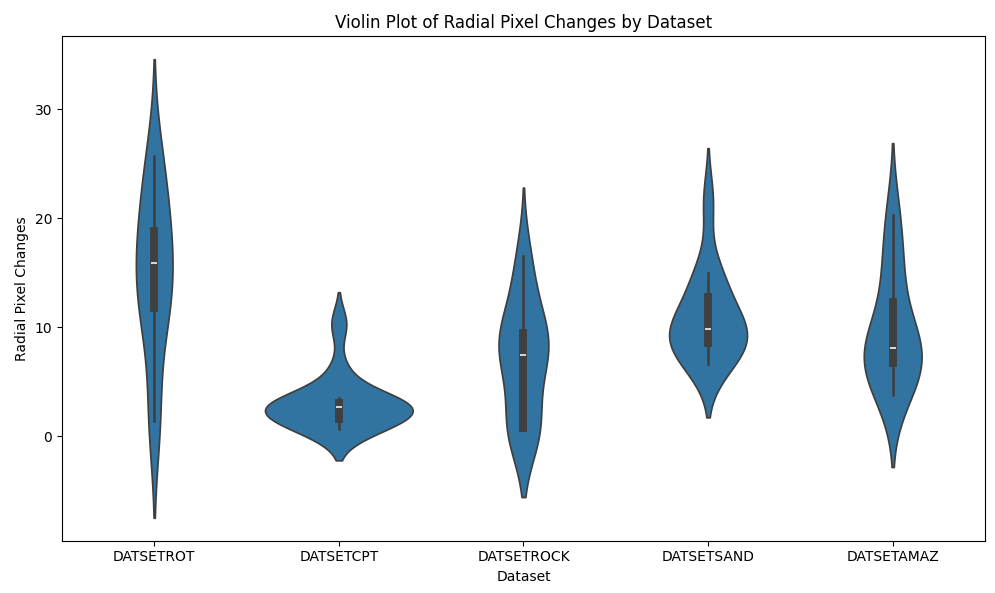
\includegraphics[width=0.8\textwidth]{Chapter 5/RESULTPLOTS/violindatasets.png}
    \caption{Heatmap of Pixel Deviations in X and Y Directions}
    \label{fig:Heatmap_XY_Dev}
\end{figure}

\subsection*{Stress}

overlap: overlap is defined as the percentage of the image that is mutual in both directions. it considers the actual movement of the UAV in GPS, and this is relative then to the image size. 



x, y-overlap-mean: 86.49, 77.81
Mean_Add_Time: 0.9229025999704997, Mean_Parameter_Inference_Time: 1.8813745498657226, Mean_Location_Inference_Time: 2.1749957524813137
Var_Add_Time: 0.06328742953493222, Var_Parameter_Inference_Time: 0.08169576957992376, Var_Location_Inference_Time: 0.15846258271884292
Total Time: 51.52535653114319
Percentage Deviation: [0.92141953] %
Preprocessing Global Detector: ORB, Preprocessing Global Matcher: FLANN, Global Matching Technique: Histogram, Local Detector: AKAZE, Local Matcher: FLANN
Mean Absolute Error GPS: [6.74818937]
[9.68383017]
Mean Length of Global Keypoints: 5777.4
Mean Number of Loc good Matches: 735.0555555555555
Mean Number of Global good Matches: 590.6333333333333
Time taken to execute The Method: 52.2591 seconds





Nice looking results:
Heat map (1, 7 bin) x and y separate, and radial - X 
GPS (or not and pixel) path estimate (ADD BACK NEXT ITERATION)
dataset specific clouds - X


Now lets add errors:
1. heatmap xy dev - pixels done - see bias


2. violin plot per dataset pixels - done (percent?) - see error. Some datasets have large errors, up to 30 pixels off radial.


\section{Maximum Error Analysis and Correlation Testing}


% insert figure of heatmap pixel estimates
% insert figure of violin plot of pixel errors

\begin{figure}[H]
    \centering
    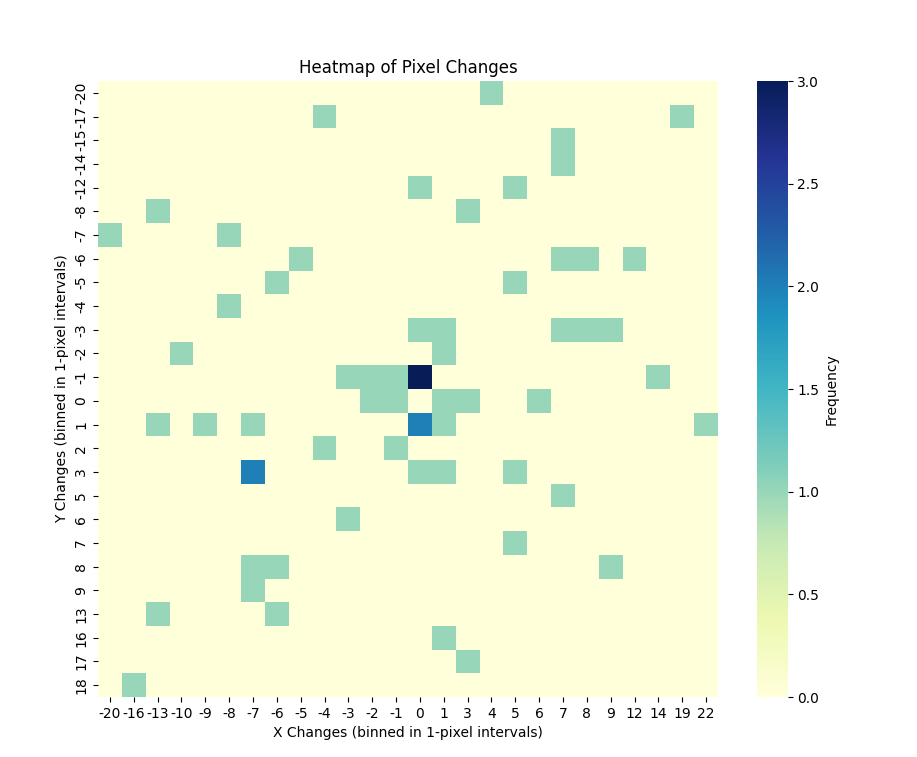
\includegraphics[width=0.8\textwidth]{Chapter 5/RESULTPLOTS/BIASPLOT_XY_HEAT.png}
    \caption{Heatmap of Pixel Deviations in X and Y Directions}
    \label{fig:Heatmap_XY_Dev}
\end{figure}


During the analysis, large variations in pixel offsets were observed in some datasets, with radial errors reaching up to 30 pixels. To investigate the source of these errors, various correlation techniques and tests were conducted between the error magnitude and potential contributing factors. These included:

\subsection{Internal Angle vs. Error Correlation}
This aimed to find if poor rotational estimations led to higher errors. A minor correlation coefficient of 0.1762 was found between angle differences and error, suggesting that the angle between the reference and inference images had an insignificant impact on localization accuracy. Thus, higher internal angles were not systematically associated with larger errors.

\subsection{Uncertainty and Error Correlation}
Correlations between error magnitude and measures of uncertainty, specifically the standard deviation and mean-median difference, were calculated. The results were as follows:

\begin{itemize}
    \item \textbf{X-axis standard deviation vs. error}: \[0.6564, 0.6572, -0.0525, 0.3039, -0.0285\]
    \item \textbf{X-axis mean-median difference vs. error}: \[-0.1352, -0.2906, 0.1642, 0.4612, 0.3105\]
    \item \textbf{Y-axis standard deviation vs. error}: \[0.6929, 0.3246, 0.0180, 0.0339, 0.0700\]
    \item \textbf{Y-axis mean-median difference vs. error}: \[-0.0422, -0.0866, -0.6616, -0.0895, -0.2613\]
\end{itemize}

These correlations showed no strong relationship between uncertainty of the method (measured by standard deviation and mean-median difference) and error. This indicates that the method was stable and consistent, and that varying errors were not primarily caused by instability in the estimation technique. This laid the foundation for considering external or practical reasons for the observed errors.

\section{Impact of Ground Truth Heading Estimation}

Upon observing a correlation between error magnitude and image sequence in the dataset, the accuracy of the estimated headings from Google Earth data was reconsidered. The initial heading estimates were generated early in the project, prior to the development of an optimized rotational estimation technique. Additionally, ground truth headings were estimated by summing internal angles, which likely introduced cumulative errors. To assess the impact of these inaccuracies, a newer, optimized pipeline was used for heading estimation, and the dataset was retested. The results showed a reduction in mean radial error from 30.37 meters to 17.91 meters, indicating that inaccurate heading estimation is a significant source of error in the system.

\section{Maximum Error Summary}

Given these findings, and the factor improvements, it is estimated that the true absolute maximum error for an individual image in the given datasets, with the ground truth data available, is in the range of 7.5-15 pixels radially. This error corresponds to around 3.4\%-6.8\% of the average radial displacement between images (220 pixels), remaining within acceptable limits for the system's design objectives. The absence of true ground truth heading data has likely amplified these errors, leading to larger observed radial deviations.















% Dataset: DATSETAMAZ
% Linear regression inferred factor x: 3.3738789378321217
% Linear regression inferred factor y: 3.455327073764407
% Interm angle: -0.0000 deg, DEV-X,Y (pixels): (-2.1586038122612763, 4.334424096596138)
% Interm angle: -195.4006 deg, DEV-X,Y (pixels): (-0.2604724435900607, -29.182543542776898)
% Interm angle: -181.0718 deg, DEV-X,Y (pixels): (-8.726932834933166, -12.225699582213906)
% Interm angle: -181.1089 deg, DEV-X,Y (pixels): (8.904814054491197, 11.030645800864932)
% Interm angle: -181.0718 deg, DEV-X,Y (pixels): (0.9801064092702632, 15.303823953695769)
% Interm angle: -181.0433 deg, DEV-X,Y (pixels): (8.748992422901125, -19.72505001809168)
% Interm angle: -3.4582 deg, DEV-X,Y (pixels): (3.2180113388305926, 15.783338928629199)
% Interm angle: -46.8223 deg, DEV-X,Y (pixels): (-26.097384699788336, 27.490768506720798)
% Interm angle: -27.1818 deg, DEV-X,Y (pixels): (20.319732604609385, 5.860656102103292)
% Interm angle: 3.2985 deg, DEV-X,Y (pixels): (-21.085862010385313, 7.309995745239746)
% Interm angle: -27.1818 deg, DEV-X,Y (pixels): (14.764122295494133, -6.466321846361325)
% Interm angle: 3.2985 deg, DEV-X,Y (pixels): (-8.075413783313135, -10.244650151048972)
% Interm angle: 20.5317 deg, DEV-X,Y (pixels): (-15.580909035827062, 21.877502015975864)

% thats metres not pixels. Max pixel is off radial is: (27.49/3.455^2 + 26.097/3.374^2 )^1/2= 12/23 (much better )